
%\section{Dynarobin leg model}

%This paper goal is to improove locomotion stability on quadrupedal robot Dynarobin, depicted in Fig. \ref{fig:Dynarobin}. 
The robot has four identical legs ($l\in \left \{ 1,2,3,4 \right \}$), each combining three rotational joints: hip, knee, and ankle, respectively. Fig. \ref{fig:DynarobinLEG} depicts one such leg, with each joint marked with a red circle and an additional mechanical spring end-effector. In order to mimic the spring-mass system, each joint controller implements impedance control \cite{citeulike:2203614}. The actual implementation goes beyond the scope of this paper and will not be further discussed. Together with adequate joint trajectory planning and inverse kinematics the legs can be tuned to mimic the behavior of an active spring-mass system \cite{conf/iros/ParkP12}\cite{6171868}, so that when the legs are in the contact with the ground, side forces and thrust forces are produced.

Besides the kinematic chain performing as an active spring, each leg contains an additional mechanical spring that changes the stiffness of the contact with the surface. Combining these mechanical springs together with leg's compliant dynamics enables us to model each leg of the robot as a single, active spring. The simplified quadruped's leg model is shown in Fig. \ref{fig:DynarobinLEG}. It consists of three masses connected by virtual active and passive springs. The passive spring has initial fixed length $L_{pl}=L_{p0}$ and parameters $K_{pl}$ and $C_{pl}$.  The actuated spring has variable parameters $K_{al}$ and $C_{al}$ and actuation is provided by changing the initial length $L_{al}=L_{a0}$ by $\Delta L$.
\begin{figure}[t!]
	\centering
	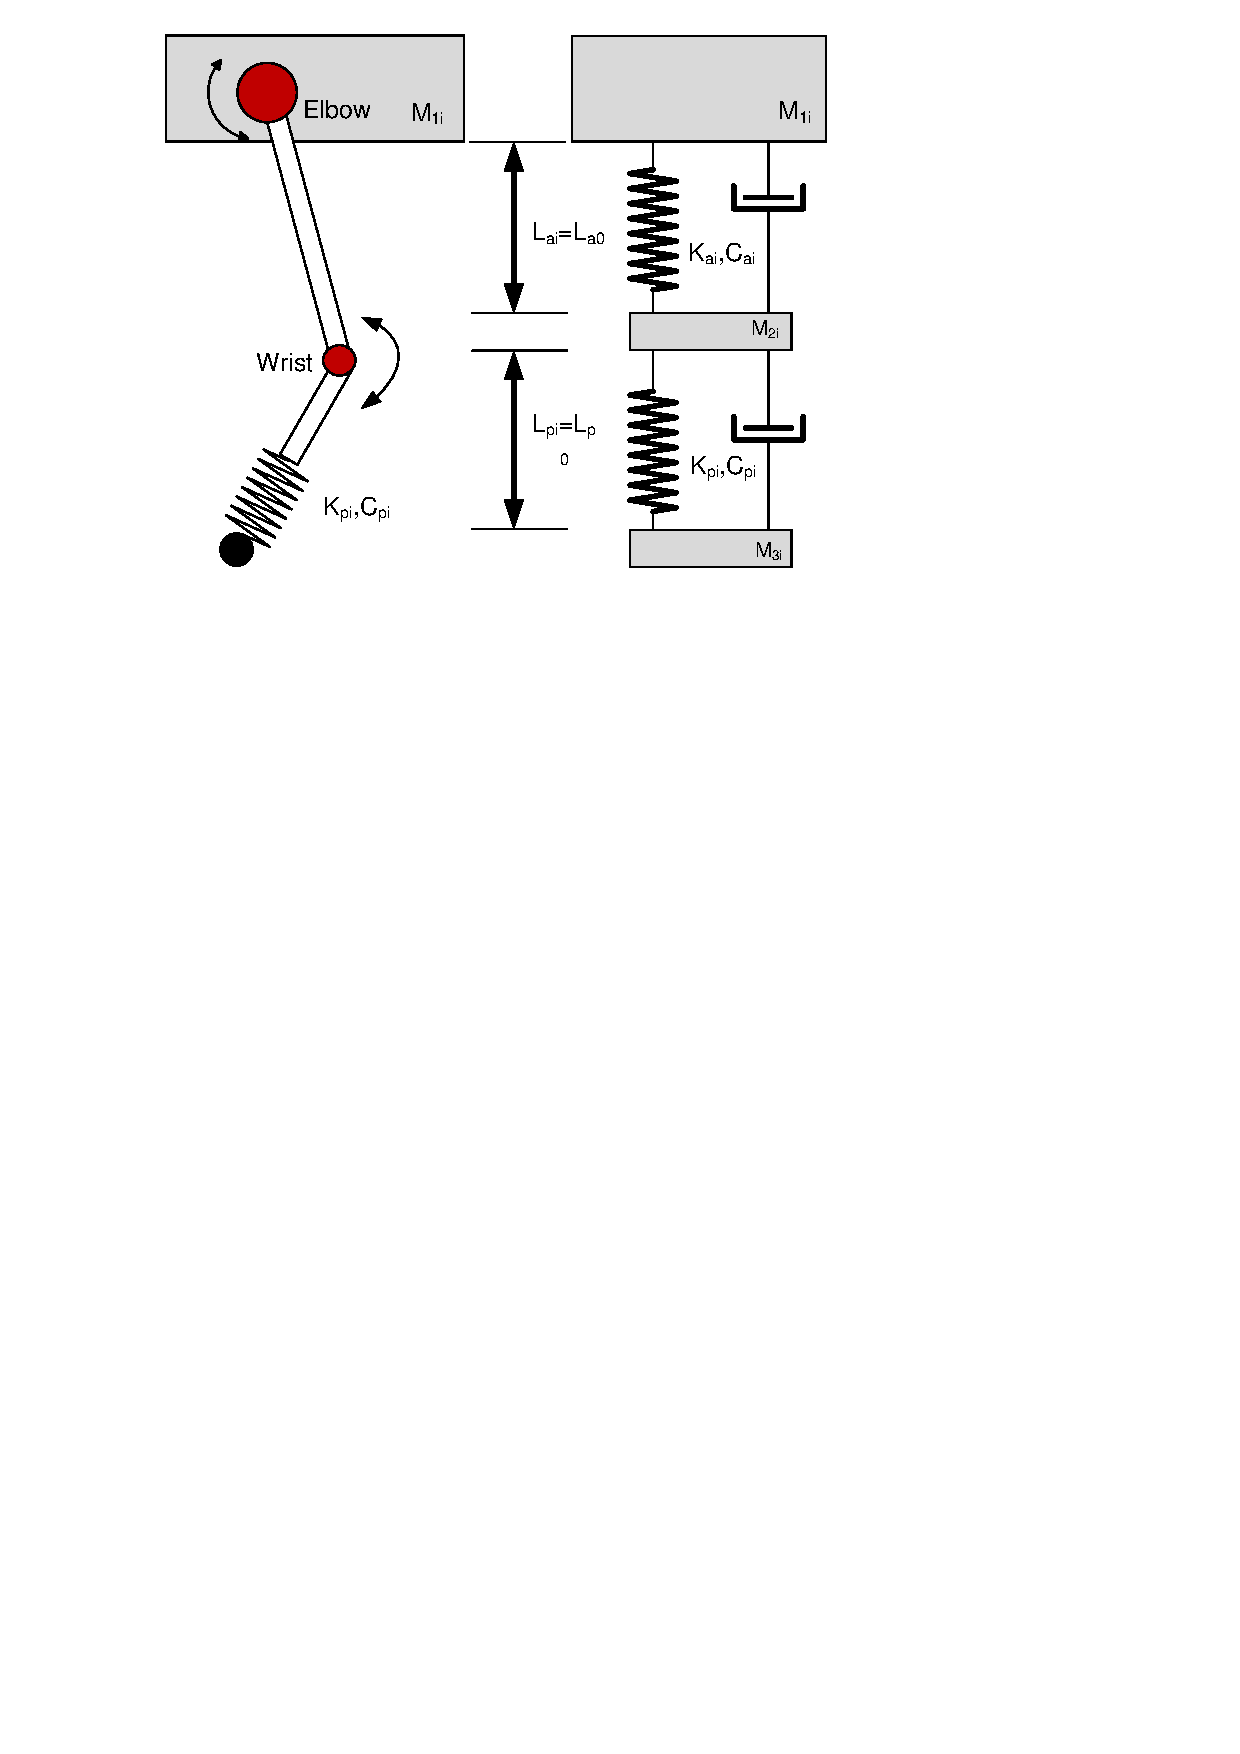
\includegraphics[width=75mm]{./pictures/Dynarobin_leg.pdf}
	\caption{Dynarobin leg model}
	\label{fig:DynarobinLEG}
\end{figure}
